\documentclass[a4paper, 12pt]{article}
\usepackage[margin=2.5cm]{geometry}
\usepackage[utf8]{inputenc}
\usepackage{amsmath}
\usepackage{amssymb}
\usepackage{graphicx}
\usepackage{hyperref}
\usepackage[square, numbers]{natbib}
\bibliographystyle{abbrvnat}

\newcommand{\unit}[1]{\,\mathrm{#1}}
\title{Cosmology}
\author{Ewan Chamberlain}
\date{Spring 2025}

\begin{document}

\maketitle

\section{Introduction}
\subsection{What is cosmology?}
From \href{https://www.google.com/search?q=cosmology+definition&sca_esv=8bb27511c7a3bbb8&ei=tNp_Z_WjLu3HhbIP0OHroQU&ved=0ahUKEwj1zcK36uiKAxXtY0EAHdDwOlQQ4dUDCBA&uact=5&oq=cosmology+definition&gs_lp=Egxnd3Mtd2l6LXNlcnAiFGNvc21vbG9neSBkZWZpbml0aW9uMgoQABiABBhGGPkBMgUQABiABDIFEAAYgAQyBRAAGIAEMgUQABiABDIFEAAYgAQyBRAAGIAEMgUQABiABDIFEAAYgAQyBRAAGIAESJsdUMoDWIMccAV4AZABAJgBW6ABmgiqAQIxNbgBA8gBAPgBAZgCFKAC7QjCAgoQABiwAxjWBBhHwgINEAAYgAQYsAMYQxiKBcICFRAAGIAEGLEDGEMYgwEYigUYRhj5AcICChAAGIAEGEMYigXCAgUQLhiABMICDBAAGIAEGA0YRhj5AcICBxAAGIAEGA3CAgUQIRigAcICDhAAGIAEGAoYDRhGGPkBwgIIEAAYCBgNGB6YAwCIBgGQBgqSBwIyMKAHy8IB&sclient=gws-wiz-serp}{Google}:
`The science of the origin and development of the universe.'

\href{https://en.wikipedia.org/wiki/Cosmology}{Wikipedia}:
`Cosmology is a branch of physics and metaphysics dealing with the nature of the universe, the cosmos.' 

\href{https://chatgpt.com/share/677fdb9a-5f44-800a-8106-8c645bef2ff6}{ChatGPT}:
`Cosmology is the scientific study of the universe as a whole, including its origins, evolution, structure, dynamics, and ultimate fate.'


So, what is cosmology?


Cosmology is the branch of physics studying the nature and evolution of the Universe as a whole.

\subsection{Why do we study cosmology?}
This definition may make cosmology seem pretty removed from our Earthly experiences, so you may be asking \textbf{why do we care?}


There are many reasons why cosmologists spend their time on the field, including:
\begin{itemize}
    \item Discovering new physics
    \begin{itemize}
        \item[--] Dark matter
        \item[--] Dark energy
    \end{itemize}
    \item Testing fundamental physics
    \begin{itemize}
        \item[--] General relativity on the largest scales
        \item[--] Baryon asymmetry
        \item[--] Neutrino mass
    \end{itemize}
    \item Philosophical
    \begin{itemize}
        \item[--] Why does the Universe look as it does?
        \item[--] Why are do we live in a Universe that can develop life?
    \end{itemize}
\end{itemize}

\section{The nature of the universe}
What is the nature of the universe? Let's start with some basic aspects \cite{Planck_2018}:
\begin{align*}
    \text{Age}&: 13.8 \unit{Gyr} = 4.36 \times 10^{17} \unit{s},\\
    \text{Diameter}&: 28.8 \unit{Gpc} = 8.90 \times 10^{28} \unit{cm}\footnotemark{}.
\end{align*}
These are some inconceivably large numbers, there's a catch: these are fundamentally \textit{human} units -- the second was originally a small fraction of one Earth day, and the meter a fraction of Earth's diameter, both chosen to be easily usable. This gives little intuition to the objective nature of the universe. Instead, we should consider measurements of the universe in units that are fundamental to nature.
\footnotetext{Being the oldest science, astronomy still holds onto some archaic traditions, one of which is the use of cgs.}

\subsection{Natural units}
Throughout these lectures we will be taking fixing $c=\hbar=G=k_\mathrm{B}=1$. This convention is adopted in the literature to simplify equations, as we may simply drop these terms. However, by combining the first three via dimensional analysis, we can develop a set of natural units, namely the Planck units:
\begin{align*}
    \text{Planck Time}&: t_{\mathrm{Pl}} = \sqrt{\frac{\hbar G}{c^5}},\\
    \text{Planck Length}&: \ell_{\mathrm{Pl}} = \sqrt{\frac{\hbar G}{c^3}}.
\end{align*}
In these units the universe has an age and a diameter of \cite{astropy:2022}:
\begin{align*}
    \text{Age}&: 8.03 \times 10^{60} t_{\mathrm{Pl}},\\
    \text{Diameter}&: 5.47 \times 10^{61} \ell_{\mathrm{Pl}}.
\end{align*}
So not only is the universe mind-boggingly large on human scales, but it is exceedingly large even on physical scales.

\subsection{Contents of the universe}
The universe today is built from the following components \cite{Planck_2018}:

\begin{itemize}
    \item $\lesssim 1\%$ radiation -- photons, neutrinos, relativistic particles.
    \item $\sim 4.9\%$ baryons -- protons, neutrons, electrons.
    \item $\sim 26.5\%$ dark matter -- we don't know.
    \item $\sim 68.6\%$ dark energy -- we \textit{really} don't know.
\end{itemize}

\begin{figure}
    \centering
    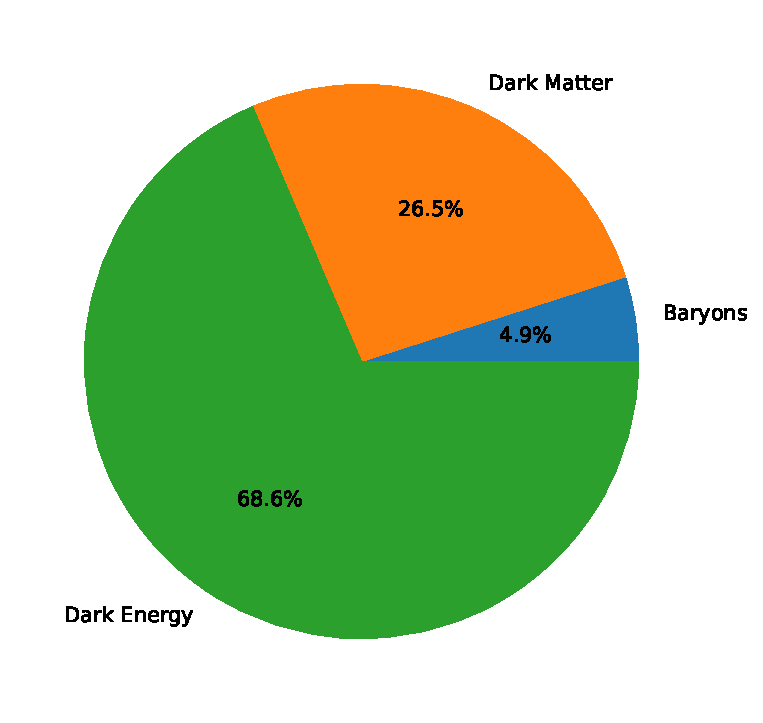
\includegraphics[width=0.8\textwidth]{universal_pie.pdf}
    \caption{Contribution of each component to the total energy density of the universe \cite{Planck_2018}. Radiation is not included as it has a small contribution.}
\end{figure}

\bibliography{ref}
\end{document}